\documentclass[aspectratio=169]{beamer}
\usepackage{beamerthemeTealOceanPdflatex} % Custom theme with oceanic colors

% Enable notes on second screen (CHANGE THIS LINE)
\setbeameroption{show notes on second screen}

\usepackage{tikz}
\usetikzlibrary{angles, quotes, shapes.geometric, arrows.meta, positioning}
\tikzstyle{block} = [rectangle, rounded corners, minimum width=3cm, minimum height=1cm,text centered, draw=black, fill=blue!10]
\tikzstyle{arrow} = [thick, ->, >=Stealth]

% Additional packages for better presentation
\usepackage{booktabs}
\usepackage{amsmath}
\usepackage{amssymb}

% Custom commands for consistency
\newcommand{\highlight}[1]{\textbf{\color{accent2}#1}}
\newcommand{\tech}[1]{\texttt{#1}}

\title{Book Recommender using NLP}
\author{Carsten Lydeking}
\institute{Zealand Business College}
\date{Oral Exam -- AI and ML, 4th Semester}

\graphicspath{{../synopsis/figures/}}

\begin{document}

% Title slide
\begin{frame}
  \titlepage
  \note{
    \textbf{OPENING (30 seconds):}
    \begin{itemize}
      \item Good morning, I'm Carsten
      \item Book recommender using NLP for oral exam
      \item 10 min presentation + questions
      \item Focus on concepts and implementation
    \end{itemize}
  }
\end{frame}

% Main presentation slides
\begin{frame}{Motivation and Problem}
\begin{itemize}
  \item Increasing demand for privacy-preserving, local-first ML applications.
  \item Typical recommender systems rely on cloud APIs and user profiles.
  \item Goal: explore feasibility of a fully offline, content-based book recommender system.
  \item Research question:
    \begin{quote}
    How can a local ML model be used to recommend books based on natural language descriptions?
    \end{quote}
\end{itemize}
\end{frame}
\begin{frame}{Architecture Overview}
\begin{columns}[T]
  \begin{column}{0.40\textwidth}
    Modular, fully local processing pipeline:
    \begin{center}
      \begin{itemize}
        \item Data cleaning and augmentation
        \item Category inference via zero-shot classification + fallback
        \item Sentence embedding with MiniLM
        \item Fast vector similarity search with FAISS
        \item Offline UI built with Streamlit
      \end{itemize}
    \end{center}
  \end{column}
  
  \begin{column}{0.55\textwidth}
    \begin{center}
      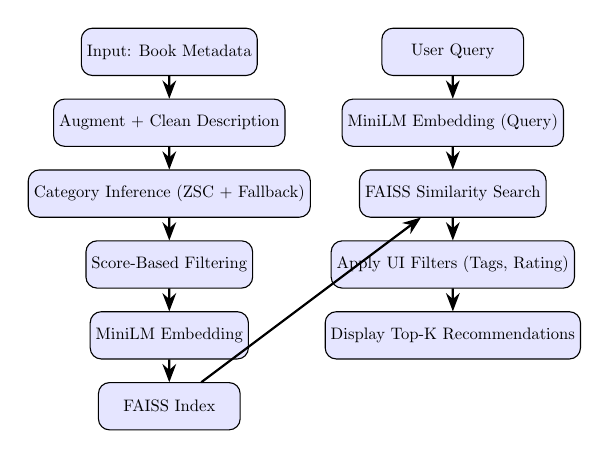
\begin{tikzpicture}[node distance=1.5cm, scale=0.60, transform shape]
        \node (desc) [block] {Input: Book Metadata};
        \node (augment) [block, below of=desc] {Augment + Clean Description};
        \node (classify) [block, below of=augment] {Category Inference (ZSC + Fallback)};
        \node (filtering) [block, below of=classify] {Score-Based Filtering};

        \node (embed) [block, below of=filtering] {MiniLM Embedding};
        \node (index) [block, below of=embed] {FAISS Index};

        \node (query) [block, right of=desc, xshift=4.5cm] {User Query};
        \node (qembed) [block, below of=query] {MiniLM Embedding (Query)};
        \node (search) [block, below of=qembed] {FAISS Similarity Search};
        \node (refine) [block, below of=search] {Apply UI Filters (Tags, Rating)};
        \node (output) [block, below of=refine] {Display Top-K Recommendations};

        \draw [arrow] (desc) -- (augment);
        \draw [arrow] (augment) -- (classify);
        \draw [arrow] (classify) -- (filtering);
        \draw [arrow] (filtering) -- (embed);
        \draw [arrow] (embed) -- (index);

        \draw [arrow] (query) -- (qembed);
        \draw [arrow] (qembed) -- (search);
        \draw [arrow] (index) -- (search);
        \draw [arrow] (search) -- (refine);
        \draw [arrow] (refine) -- (output);
      \end{tikzpicture}
    \end{center}
  \end{column}
\end{columns}
\end{frame}
\begin{frame}{Dataset Exploration}
  
\begin{columns}[T]
  \centering
  \begin{column}{0.49\textwidth}
    Original dataset $\sim$ 6800 books
    \begin{itemize}
          \item Missing or inconsistent fields (authors, categories, descriptions)
          \item Very short or low-quality descriptions
          \item Category noise across sources
          \item OpenLibrary and Google Books API used to enrich metadata
          \item Rows with $<9$ words in description removed
          \item Final dataset: 5160 high-confidence books
        \end{itemize}
  \end{column}

  \begin{column}{0.49\textwidth}
  \centering
      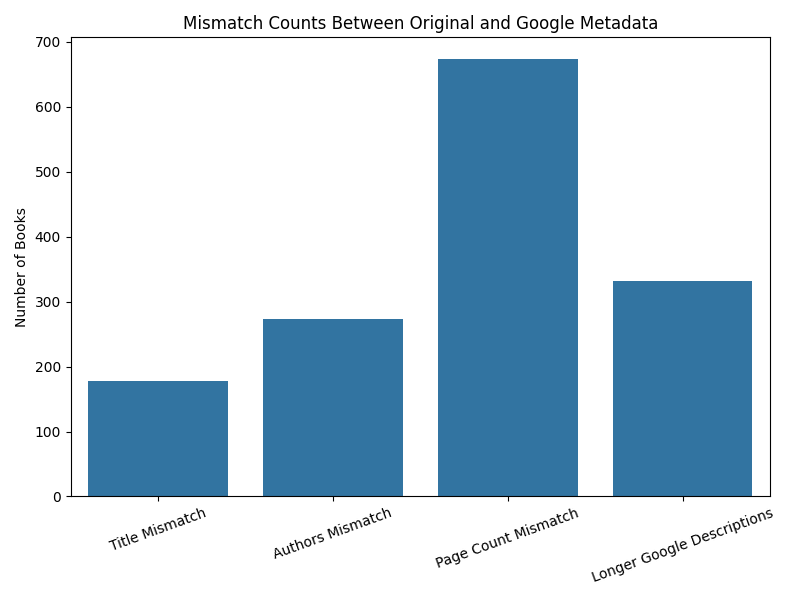
\includegraphics[width=\textwidth]{reexp_mismatch_counts.png}
  \end{column}
\end{columns}
\end{frame}
\begin{frame}{Category Inference}

\begin{columns}
  % First column with text and bullet points
  \begin{column}{0.49\textwidth}
    \centering
    \begin{itemize}
      \item Zero-shot classification with BART-MNLI
      \item 13 candidate categories defined
      \item Fallback keyword rules added for weak predictions
      \item Per-category metrics calculated:
        \begin{itemize}
          \item Precision
          \item Recall
          \item F1-score
        \end{itemize}

      \item Final filtering based on confidence thresholds:
        \begin{itemize}
          \item description\_length $\geq$ 200 chars
          \item avg\_score $\geq$ 0.2
          \item max\_score $\geq$ 0.4
        \end{itemize}
  \end{itemize} 
  \end{column}

  \begin{column}{0.45\textwidth}
    \centering
    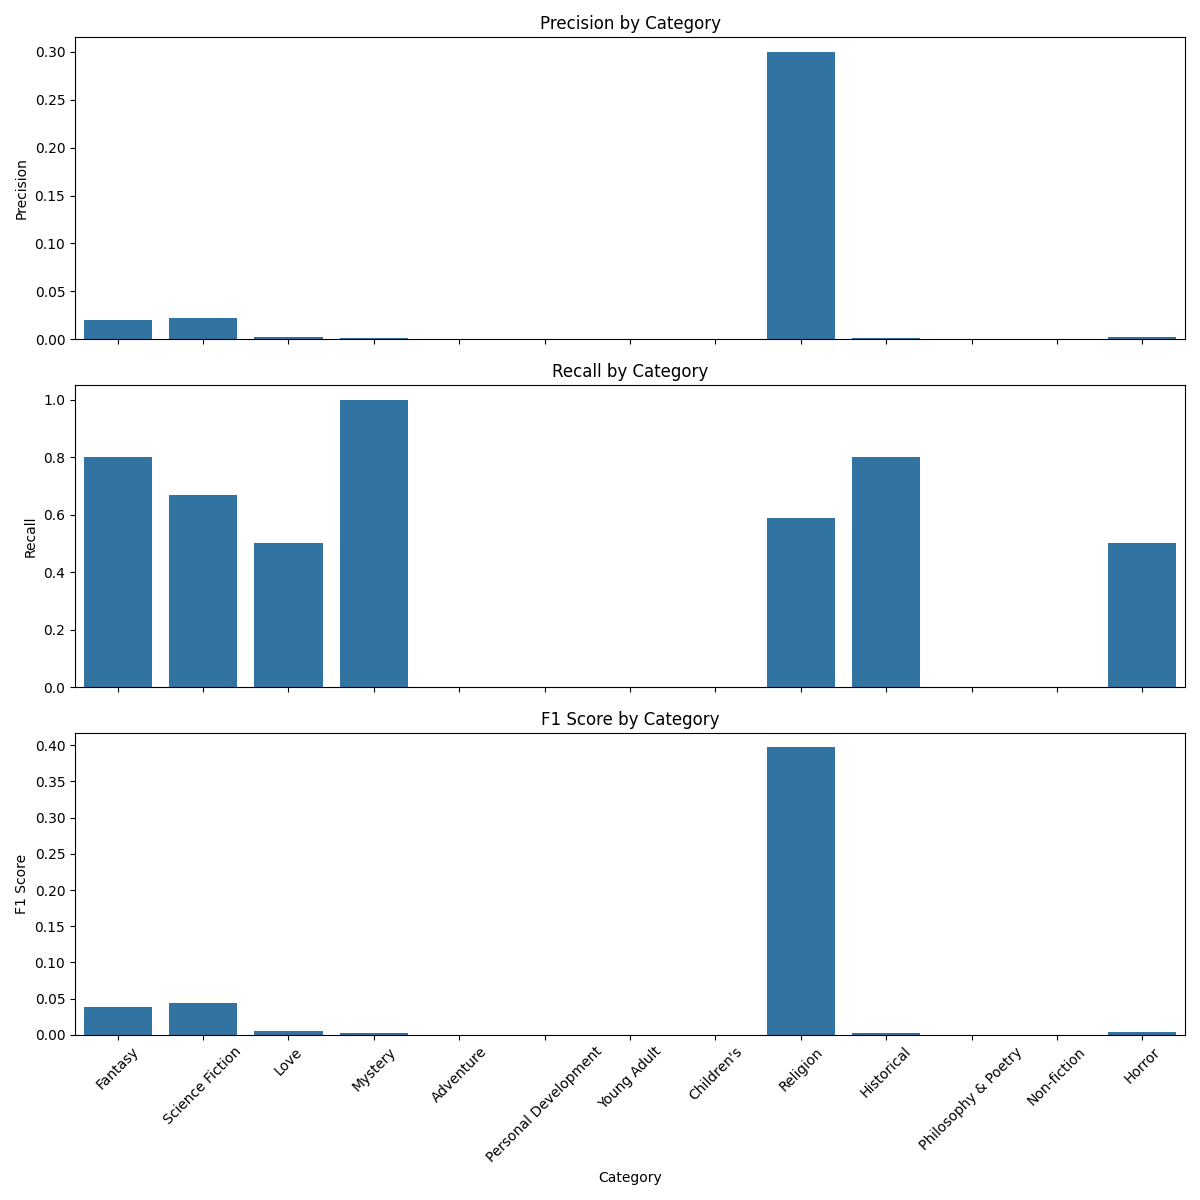
\includegraphics[width=\textwidth]{refine_category_metrics_plot.png}
  \end{column}
\end{columns}

\end{frame}

\begin{frame}{Semantic Embedding \& Vector Search}

\begin{columns}[T]
  \begin{column}{0.50\textwidth}
    \textbf{Sentence Embedding with \tech{MiniLM}:}
    \begin{itemize}
      \item \highlight{Model:} \tech{all-MiniLM-L6-v2}
      \item \highlight{Input format:}
        {\scriptsize \textit{"Title: ... Author: ... Description: ..."}}
      \item \highlight{Output:} 384-dimensional vectors
      \item \highlight{Advantage:} Semantic similarity beyond keywords
    \end{itemize}

    \vspace{0.3cm}
    \textbf{Vector Search with \tech{FAISS}:}
    \begin{itemize}
      \item \highlight{Index:} 5,160 book embeddings
      \item \highlight{Search:} L2 distance (exact search)
      \item \highlight{Performance:} $<$ 10ms query time
      \item \highlight{Local:} No external dependencies
    \end{itemize}

	\vspace{0.2cm}
    \textbf{Why \tech{MiniLM} Specifically:}
    \begin{itemize}
        \item Balance of performance vs size
        \item Small enough to run locally in real-time
        \item But powerful enough for semantic understanding
    \end{itemize}

  \end{column}

  \begin{column}{0.45\textwidth}
    \centering
    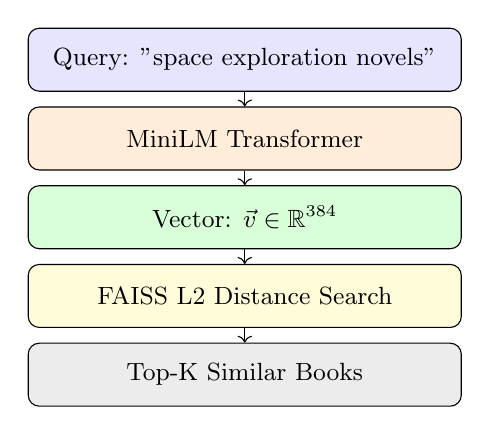
\begin{tikzpicture}[node distance=1.0cm, every node/.style={font=\small}]
        % Embedding process
        \node (input) [draw, rounded corners, minimum width=5.5cm, minimum height=0.8cm, fill=blue!10] 
        {\small Query: "space exploration novels"};

        \node (embed) [below of=input, draw, rounded corners, minimum width=5.5cm, minimum height=0.8cm, fill=orange!15] 
        {\small MiniLM Transformer};

        \node (vector) [below of=embed, draw, rounded corners, minimum width=5.5cm, minimum height=0.8cm, fill=green!15] 
        {\small Vector: $\vec{v} \in \mathbb{R}^{384}$};

        % Search process
        \node (faiss) [below of=vector, draw, rounded corners, minimum width=5.5cm, minimum height=0.8cm, fill=yellow!15] 
        {\small FAISS L2 Distance Search};

        \node (results) [below of=faiss, draw, rounded corners, minimum width=5.5cm, minimum height=0.8cm, fill=gray!15] 
        {\small Top-K Similar Books};

        % Arrows
        \draw[->] (input) -- (embed);
        \draw[->] (embed) -- (vector);
        \draw[->] (vector) -- (faiss);
        \draw[->] (faiss) -- (results);
    \end{tikzpicture}
    
    \vspace{0.2cm}
    \small \textit{End-to-end semantic search in $<$ 200ms}
  \end{column}
\end{columns}

\end{frame}

\note{
	\begin{columns}[T]
    	\begin{column}{0.49\textwidth}
			[TIMING: 1.5 min Embeddings - CORE TECHNICAL SLIDE]
			\begin{itemize}
			  \item "Embeddings convert text to numbers that capture meaning - 384 dimensions means each book becomes a point in 384D space"
			  \item "Books with similar meanings cluster together in this space -Like a map where distance represents semantic similarity"
			\end{itemize}
			
			\vspace{0.1cm}
			[CONCRETE EXAMPLE (use the diagram):]
			\begin{itemize}
			  \item "User types 'space exploration novels' - MiniLM converts this to 384 numbers"
			  \item "FAISS finds books whose embeddings are closest"
			  \item "Might find 'Mars colonization story', 'astronaut memoir' - no exact keyword matches needed!"
			\end{itemize}
			
			\vspace{0.1cm}
			[PERFORMANCE EMPHASIS:]
			\begin{itemize}
			  \item "Sub-200ms total - feels instant to users"
			  \item "Most time in embedding query, search is nearly instant"
			  \item "Scales well - current dataset tiny compared to FAISS capabilities"
			\end{itemize}
			\end{column}
			
			\begin{column}{0.49\textwidth}
			[TECHNICAL DEPTH (if asked):]
			\begin{itemize}
			  \item "Could use cosine similarity but L2 works well for normalized embeddings"
			  \item "FAISS uses optimized algorithms for billion-scale search"
			  \item "IndexFlatL2 = exact search, could use approximate for speed"
			\end{itemize}
			
			\vspace{0.1cm}
			[POTENTIAL QUESTIONS:]
			\begin{itemize}
			  \item \textit{"Why not larger models like BERT?"} → "Size vs performance tradeoff - need to run locally"
			  \item \textit{"How does semantic similarity work?"} → "Model trained to put similar meanings close together in vector space"
			  \item \textit{"What if user query very different from training?"} → "May not work well - limitation of current approach"
			  \item \textit{"Could you use approximate search?"} → "Yes, FAISS has IVF, LSH options for speed vs accuracy tradeoff"
			\end{itemize}
			
			\vspace{0.1cm}
			[TRANSITION:]
			\begin{itemize}
			  \item "Let me show you how this looks in the actual user interface..."
			\end{itemize}
    \end{column}
  \end{columns}
}

\begin{frame}{Vector Similarity Search with FAISS}

\begin{columns}[T]
  \begin{column}{0.55\textwidth}
    \begin{itemize}
        \item Used \textbf{Facebook AI Similarity Search (FAISS)} library which performs L2 (Euclidean) distance search in embedding space
        \item Index built with:
          \begin{itemize}
            \item 5160 book embeddings (\( \vec{v} \in \mathbb{R}^{384} \))
            \item Exact search (IndexFlatL2)
          \end{itemize}
        \item At runtime:
          \begin{itemize}
            \item User query is embedded
            \item Top-k nearest neighbors retrieved
            \item Results shown in UI
            \item \textbf{Fully local}, fast search
          \end{itemize}
        \item Example Queries
          \begin{itemize}
            \item "Instead of 'fantasy dragons', user can type 'books about magical creatures'"
            \item "'philosophical science fiction' finds books exploring deep questions"
            \item "'unreliable narrator mystery' - semantic understanding of literary techniques"
          \end{itemize}
    \end{itemize}
  \end{column}

  \begin{column}{0.40\textwidth}
    \centering
    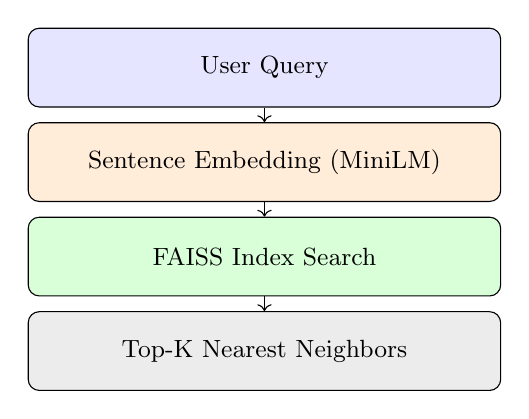
\begin{tikzpicture}[node distance=1.2cm, every node/.style={font=\small}]
        \node (query) [draw, rounded corners, minimum width=6cm, minimum height=1cm, fill=blue!10] {User Query};

        \node (embed) [below of=query, draw, rounded corners, minimum width=6cm, minimum height=1cm, fill=orange!15] {Sentence Embedding (MiniLM)};

        \node (faiss) [below of=embed, draw, rounded corners, minimum width=6cm, minimum height=1cm, fill=green!15] {FAISS Index Search};

        \node (results) [below of=faiss, draw, rounded corners, minimum width=6cm, minimum height=1cm, fill=gray!15] {Top-K Nearest Neighbors};

        \draw[->] (query) -- (embed);
        \draw[->] (embed) -- (faiss);
        \draw[->] (faiss) -- (results);
    \end{tikzpicture}
  \end{column}
\end{columns}

\end{frame}

\note{
  \begin{columns}[T]
    \begin{column}{0.49\textwidth}
      [TIMING: 1 minute - DEMO THE INTERFACE (point to screenshot):]
      \begin{itemize}
        \item "Simple, clean interface built with Streamlit"
        \item "User types natural language - no complex syntax"
        \item "Results appear instantly with covers and descriptions"
        \item "Can filter by genre, sort by rating"
      \end{itemize}

      \vspace{0.2cm}
      [PRIVACY AND INDEPENDENCE EMPHASIS:]
      \begin{itemize}
        \item "No data ever leaves the user's device - No tracking cookies, no user profiles, no analytics"
        \item "User has complete control - can run offline"
        \item "Contrast with Amazon, Goodreads - they track everything"
      \end{itemize}
      
      \vspace{0.2cm}
      [TECHNICAL IMPLEMENTATION:]
      \begin{itemize}
        \item "Streamlit chosen for rapid prototyping"
        \item "Could be ported to web app, mobile app, desktop app"
        \item "All processing happens in Python backend"
        \item "UI just displays results, no smart client needed"
      \end{itemize}
    \end{column}
    
    \begin{column}{0.49\textwidth}
      [PERFORMANCE DETAILS:]
      \begin{itemize}
        \item "200ms feels instant to users"
        \item "Most delay is loading book cover images"
        \item "Could optimize with image caching, lazy loading"
        \item "Runs smoothly on 4GB RAM laptop"
      \end{itemize}
      
      \vspace{0.2cm}
      [POTENTIAL QUESTIONS:]
      \begin{itemize}
        \item \textit{"Could this scale to millions of books?"} → "Yes, FAISS designed for billion-scale, just need more RAM"
        \item \textit{"What about mobile deployment?"} → "Would need model quantization, smaller embedding dimension"
        \item \textit{"How update book database?"} → "Currently manual, could automate with book APIs"
        \item \textit{"Could users add their own books?"} → "Yes, just run embedding pipeline on new books"
      \end{itemize}
      
      \vspace{0.2cm}
      [TRANSITION:]
      \begin{itemize}
        \item "To reflect on the project, we can consider the following aspects..."
      \end{itemize}
    \end{column}
  \end{columns}
}

\begin{frame}{Critical Analysis \& Future Directions}

\begin{columns}[T]
  \begin{column}{0.50\textwidth}
    \textbf{Implementation Strengths:}
    \begin{itemize}
      \item \highlight{Privacy-preserving} by design
      \item \highlight{Semantic understanding} beyond keyword matching
      \item \highlight{Lightweight} - runs on consumer hardware
      \item \highlight{Modular architecture} for easy extension
    \end{itemize}

    \vspace{0.3cm}
    \textbf{Current Limitations:}
    \begin{itemize}
      \item \highlight{No personalization} - stateless by design
      \item \highlight{Dataset scope} - 5,160 books vs. commercial scale
      \item \highlight{Cold start problem} for new books
      \item \highlight{No feedback learning} - static recommendations
    \end{itemize}

    \vspace{0.3cm}
    \textbf{Edge AI:}
      \begin{itemize}
        \item Edge AI is popular term for local-first ML
        \item Growing trend in mobile, home, IoT, privacy applications
        \item The project fits this paradigm perfectly
      \end{itemize}
  \end{column}

  \begin{column}{0.45\textwidth}
    \textbf{Future Research Directions:}
    \begin{itemize}
      \item \highlight{Hybrid approach:} Combine content-based with collaborative filtering
      \item \highlight{Better embeddings:} Experiment with domain-specific models
      \item \highlight{Privacy-preserving personalization:} Local user preference learning
      \item \highlight{Multi-modal features:} Include cover images, genre embeddings
    \end{itemize}

    \begin{center}
    \begin{beamercolorbox}[sep=8pt,center,rounded=true]{block body}
    \scriptsize \textit{"Demonstrates that local-first ML - or using a more popular term - edge AI, can provide meaningful semantic recommendations without compromising user privacy or requiring cloud infrastructure."}
    \end{beamercolorbox}
    \end{center}
  \end{column}
\end{columns}

\note{
  \begin{columns}[T]
    \begin{column}{0.49\textwidth}
      [TIMING: 1 minute - HONEST SELF-ASSESSMENT:]
      \begin{itemize}
        \item "This is proof-of-concept, not production system"
        \item "Goal was to demonstrate feasibility, not perfection - Garbage In, Garbage Out"
      \end{itemize}
      
      \vspace{0.1cm}
      [LIMITATIONS:]
      \begin{itemize}
        \item "No personalization - everyone gets same results for same query"
        \item "Dataset small compared to Amazon's millions of books"
        \item "New books need manual addition and embedding - batch trained"
      \end{itemize}
      
      \vspace{0.1cm}
      [FUTURE DIRECTIONS:]
      \begin{itemize}
        \item "Hybrid: Add collaborative filtering while preserving privacy and independence"
        \item "Better embeddings: Fine-tune MiniLM on book-specific corpus"
        \item "Local personalization: Session-based learning without tracking"
        \item "Multi-modal: Computer vision on book covers for genre signals"
      \end{itemize}
    \end{column}
    
    \begin{column}{0.49\textwidth}

      [POTENTIAL QUESTIONS:]
      \begin{itemize}
        \item \textit{"How would you add personalization?"} → "Local preference vectors, federated learning, session-based adaptation"
        \item \textit{"Could this work for other domains?"} → "Yes - movies, music, research papers, any content with descriptions"
        \item \textit{"What's the biggest technical limitation?"} → "Embedding quality for domain-specific queries"
        \item \textit{"How evaluate recommendation quality?"} → "User studies, semantic similarity benchmarks, domain expert evaluation"
      \end{itemize}
      
      \vspace{0.2cm}
      [TRANSITION:]
      \begin{itemize}
        \item "Let me conclude by answering the original research question..."
      \end{itemize}
    \end{column}
  \end{columns}
}

\end{frame}
\begin{frame}{Conclusion}

\begin{columns}[T]
  \begin{column}{0.45\textwidth}
    \textbf{Research Question Answered:}
    \begin{center}
    \begin{beamercolorbox}[sep=1pt,center,rounded=true]{block title}
    \scriptsize \textit{How can a local ML model recommend books based on natural language descriptions?}
    \end{beamercolorbox}
    \end{center}

    \textbf{Solution Implemented:}
    \begin{itemize}
      \item \highlight{Semantic embeddings} with MiniLM transformers
      \item \highlight{Vector similarity search} using FAISS
      \item \highlight{Zero-shot classification} for categorization
      \item \highlight{Privacy-first design} - fully local processing
      \item \highlight{Key Contributions:} \textit{Proof-of-concept that modern NLP enables practical, privacy-preserving recommendation systems}
    \end{itemize}
  \end{column}

  \begin{column}{0.50\textwidth}
    \centering
    \textbf{System Architecture:}
    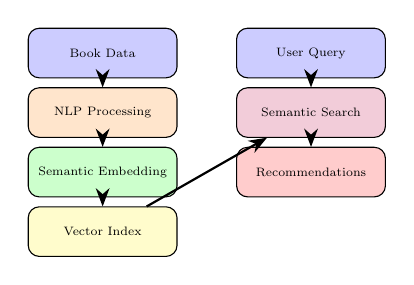
\begin{tikzpicture}[node distance=1.2cm, scale=0.9, every node/.style={font=\scriptsize}, scale=0.7, transform shape]
    % Simplified final architecture
    \node (data) [block, fill=blue!20] {Book Data};
    \node (process) [block, below of=data, fill=orange!20] {NLP Processing};
    \node (embed) [block, below of=process, fill=green!20] {Semantic Embedding};
    \node (index) [block, below of=embed, fill=yellow!20] {Vector Index};
    
    \node (query) [block, right of=data, xshift=3cm, fill=blue!20] {User Query};
    \node (search) [block, below of=query, fill=purple!20] {Semantic Search};
    \node (results) [block, below of=search, fill=red!20] {Recommendations};

    \draw [arrow] (data) -- (process);
    \draw [arrow] (process) -- (embed);
    \draw [arrow] (embed) -- (index);
    \draw [arrow] (query) -- (search);
    \draw [arrow] (index) -- (search);
    \draw [arrow] (search) -- (results);
    \end{tikzpicture}

    \vspace{0.4cm}
    \textbf{Impact \& Applications:}
    \begin{itemize}
      \item Educational tool for privacy-aware ML
      \item Foundation for local-first recommendation systems
      \item Demonstrates transformer accessibility on consumer hardware
    \end{itemize}
  \end{column}
\end{columns}

\end{frame}
\begin{frame}{End of Presentation}
  \centering
    \Large Thank you for your attention!
    \vspace{0.1cm}
    \begin{center}
        
\includegraphics[scale=0.4]{figures/tm-logo-nobg-quarter.png}
    \end{center}
    \Large Questions?
\end{frame}

% Backup slides for Q&A
\begin{frame}{Backup: Per-Category Metrics}

\begin{center}
  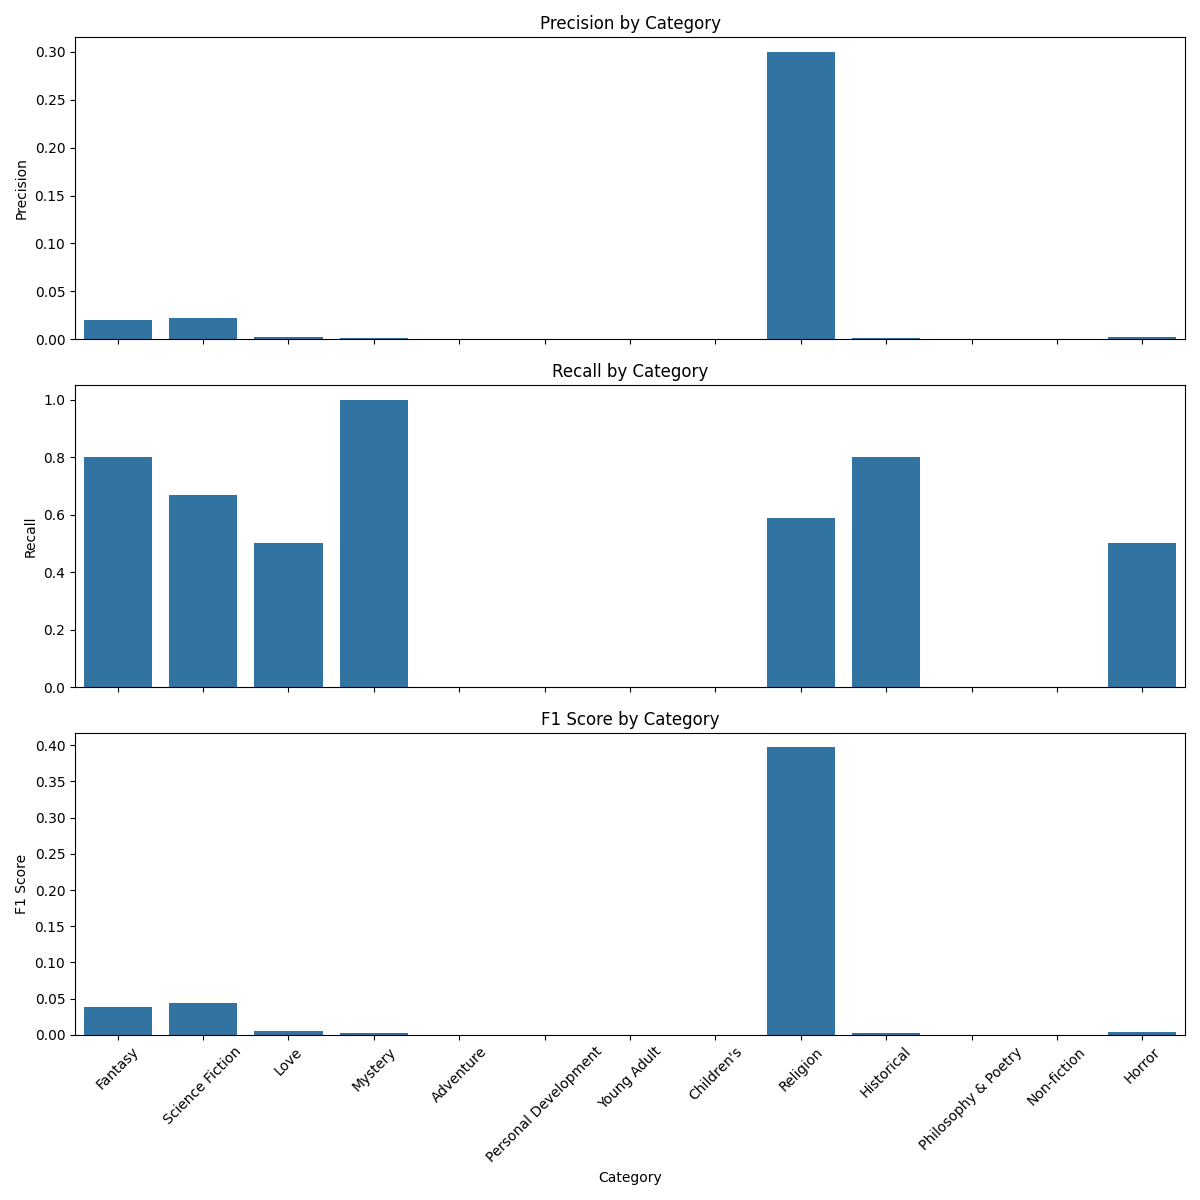
\includegraphics[width=0.45\textwidth]{refine_category_metrics_plot.png}
\end{center}

\end{frame}

\begin{frame}{Backup: Fallback Keywords}

\begin{itemize}
    \item Fallback used when zero-shot model confidence was low
    \item Example keywords:
    \begin{itemize}
        \item \textbf{Fantasy}: magic, wizard, dragon
        \item \textbf{Science Fiction}: space, AI, dystopia
        \item \textbf{Love}: romance, passion, relationship
        \item \textbf{Mystery}: detective, clue, crime
        % Add more if you like
    \end{itemize}
\end{itemize}

\end{frame}

\begin{frame}{Backup: Performance}

\begin{itemize}
    \item Embedding time per book: $\approx$ 2 ms (batch embedding)
    \item Query embedding: $\approx$ 50-200 ms
    \item FAISS search: $<$ 10 ms
    \item UI render time: $\approx$ 1-2 seconds (including image loading)
    \item All processing fully local on consumer-grade laptop
\end{itemize}

\end{frame}

\begin{frame}{Backup: Concrete Examples}

\begin{columns}[T]
  \begin{column}{0.50\textwidth}
    \textbf{Example Query 1:}
    \begin{beamercolorbox}[sep=4pt,left]{block body}
     \textit{"Books about artificial intelligence and ethics"}
    \end{beamercolorbox}
    
    \textbf{Top Results:}
    \begin{itemize}
      \item  "The Alignment Problem" - Brian Christian
      \item  "Life 3.0" - Max Tegmark  
      \item  "Weapons of Math Destruction" - Cathy O'Neil
    \end{itemize}

    \vspace{0.1cm}
    \textbf{Example Query 2:}
    \begin{beamercolorbox}[sep=4pt,left]{block body}
     \textit{"mystery novels with unreliable narrators"}
    \end{beamercolorbox}
    
    \textbf{Top Results:}
    \begin{itemize}
      \item  "Gone Girl" - Gillian Flynn
      \item  "The Girl on the Train" - Paula Hawkins
      \item  "In the Woods" - Tana French
    \end{itemize}
  \end{column}

  \begin{column}{0.45\textwidth}
    \textbf{What This Demonstrates:}
    \begin{itemize}
      \item  \highlight{Semantic understanding} beyond keywords
      \item  \highlight{Abstract concept matching} (ethics, unreliable narrators)
      \item  \highlight{Cross-genre discovery} potential
    \end{itemize}

    \vspace{0.1cm}
    \textbf{Evaluation Challenges:}
    \begin{itemize}
      \item  No ground truth for "perfect" recommendations
      \item  Subjective nature of book preferences
      \item  \highlight{Solution:} Focus on semantic relevance rather than prediction accuracy
    \end{itemize}

    \vspace{0.1cm}
    \textbf{Discussion Starters:}
    \begin{itemize}
      \item  How could one evaluate recommendation quality
      \item  Books with sparse descriptions
      \item  Could this approach work for other domains?
    \end{itemize}
  \end{column}
\end{columns}

\end{frame}

\end{document}